\documentclass[a4paper,12pt]{article}

% Paquetes básicos
\usepackage[utf8]{inputenc}
\usepackage[T1]{fontenc}
\usepackage[spanish]{babel}
\usepackage{graphicx}
\usepackage{xcolor}
\usepackage{lipsum}
\usepackage{geometry}
\geometry{top=3cm, bottom=3cm, left=2.5cm, right=2.5cm}

% Paquetes para diseño
\usepackage{titlesec}
\usepackage{fancyhdr}
\usepackage{amsmath}
\usepackage{amssymb}
\usepackage{hyperref}

% Paquetes para el entorno lstlisting
\usepackage{listings}
\usepackage{inconsolata}

% Paquete para fondo
\usepackage{background}
\usepackage{pdfpages}

% Configuración de lstlisting
\lstset{
    language=Python,
    basicstyle=\ttfamily\small,
    keywordstyle=\color{blue}\bfseries,
    stringstyle=\color{teal},
    commentstyle=\color{gray}\itshape,
    numbers=left,
    numberstyle=\tiny\color{gray},
    backgroundcolor=\color{black!5},
    frame=single,
    rulecolor=\color{black!50},
    breaklines=true,
    captionpos=b,
    showstringspaces=false
}

% Configuración de título
\titleformat{\section}{\normalfont\Large\bfseries}{\thesection}{1em}{}

% Información del documento
\title{
    \vspace{-2cm}
    
\includegraphics[width=0.3\textwidth]{images/fccee.jpg} \\ % Cambia el logo si es necesario
    \LARGE Ingeniería Informática + ADE\\
    \large Universidad de Granada (UGR)\\[1cm]
}
\author{\textbf{Autor:} Ismael Sallami Moreno}
\date{\textbf{Asignatura:} Econometría}

% Configuración del fondo
\backgroundsetup{
    scale=1,
    color=black,
    opacity=0.2,
    angle=0,
    position=current page.south,
    vshift=0pt,
    hshift=0pt,
    contents={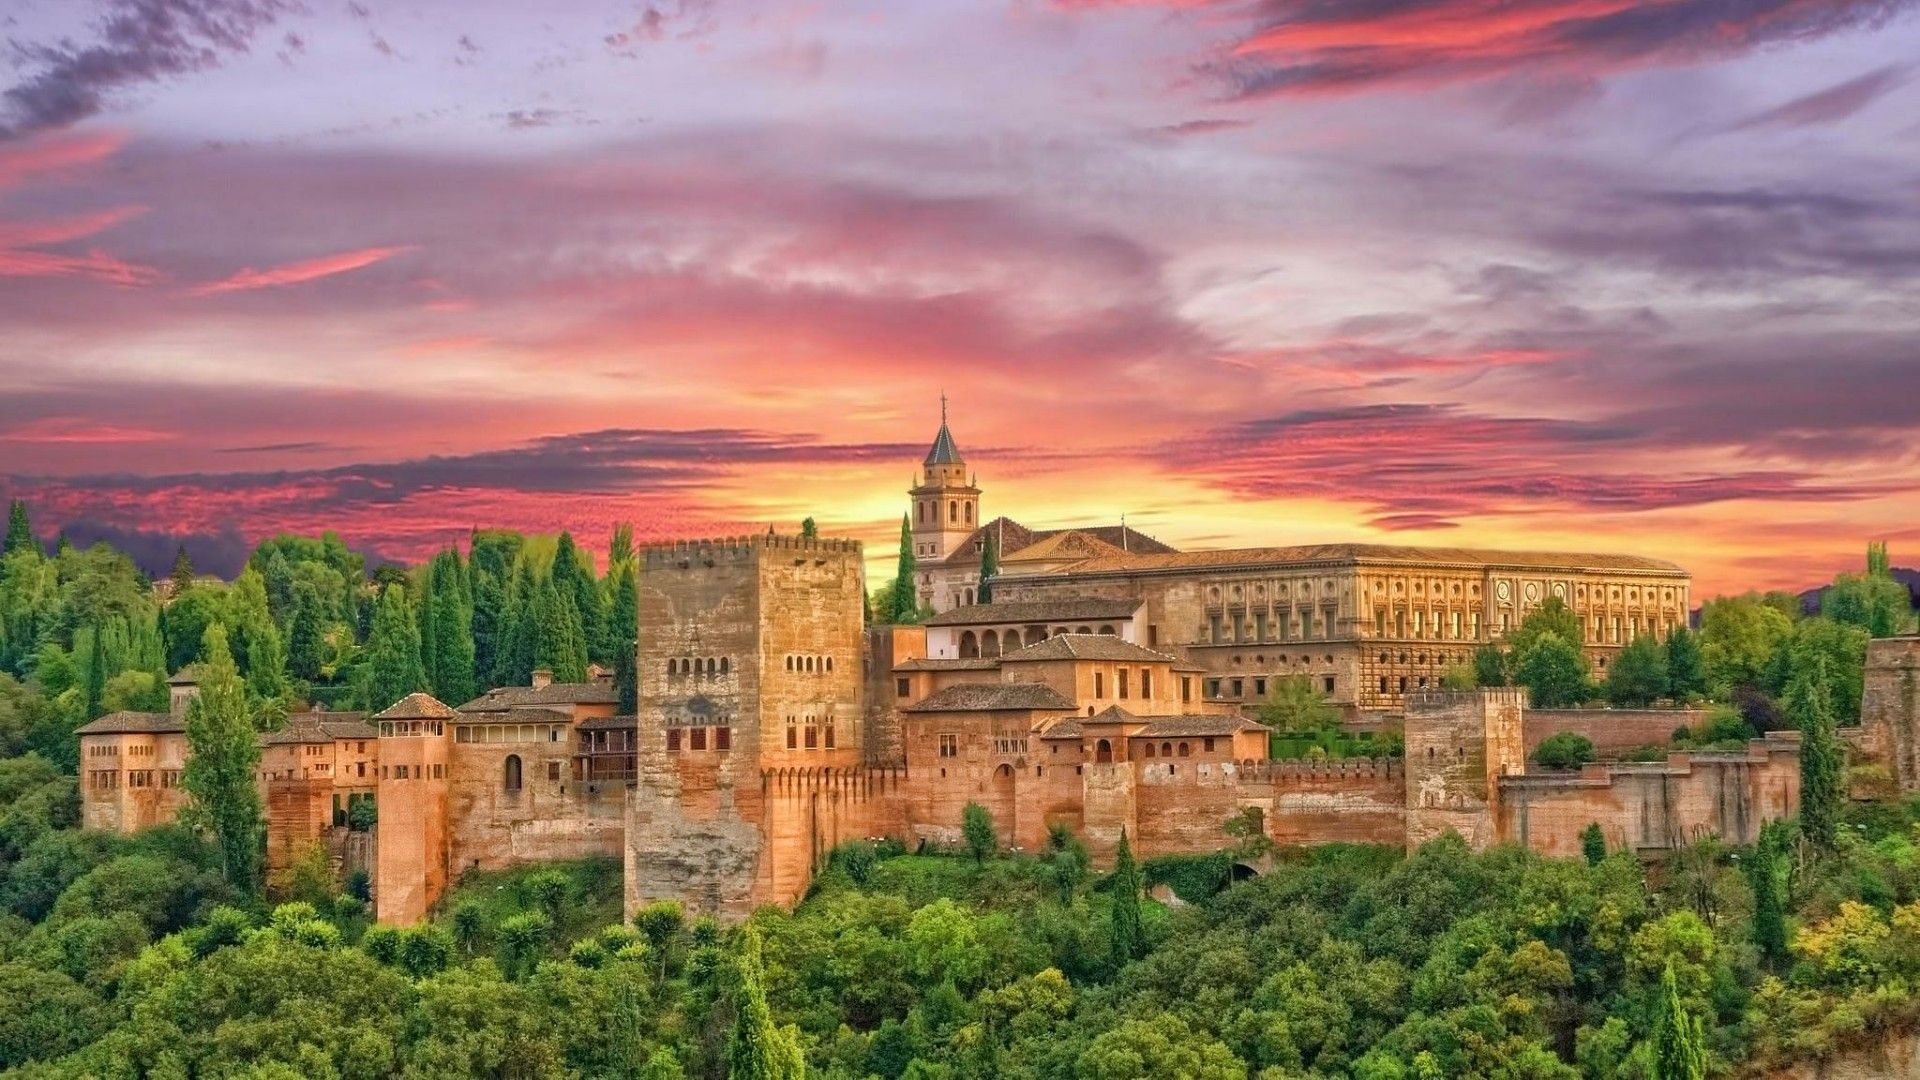
\includegraphics[width=\paperwidth,height=\paperheight,keepaspectratio]{images/granada.jpg}}
}

% Inicio del documento
\begin{document}

% Portada
\maketitle
\thispagestyle{empty}

\begin{center}
    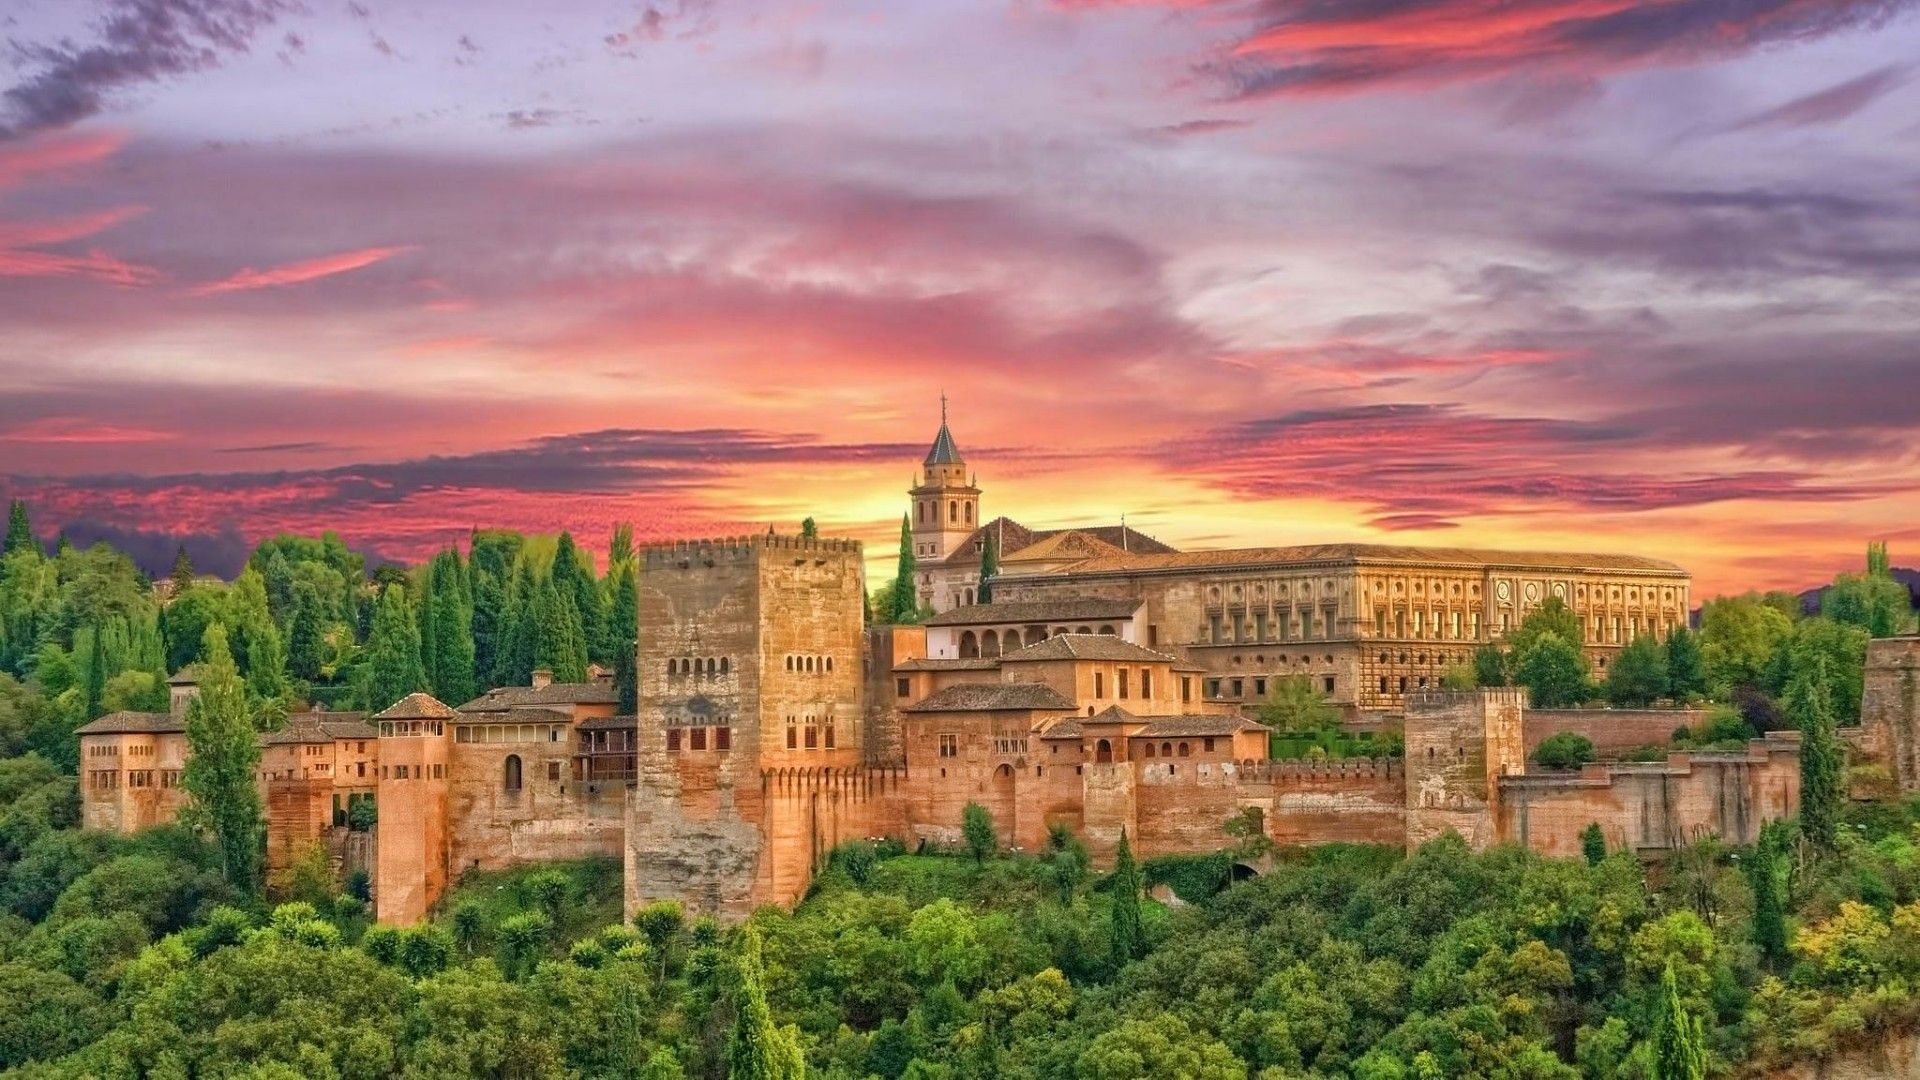
\includegraphics[width=\textwidth,height=0.4\textheight,keepaspectratio]{images/granada.jpg} \\ % Añade tu imagen de fondo
    \vfill
\end{center}

\newpage

% Índice (opcional)
\tableofcontents
\newpage

\section{Ejercicios Propuestos}
\subsection{Tema 2}
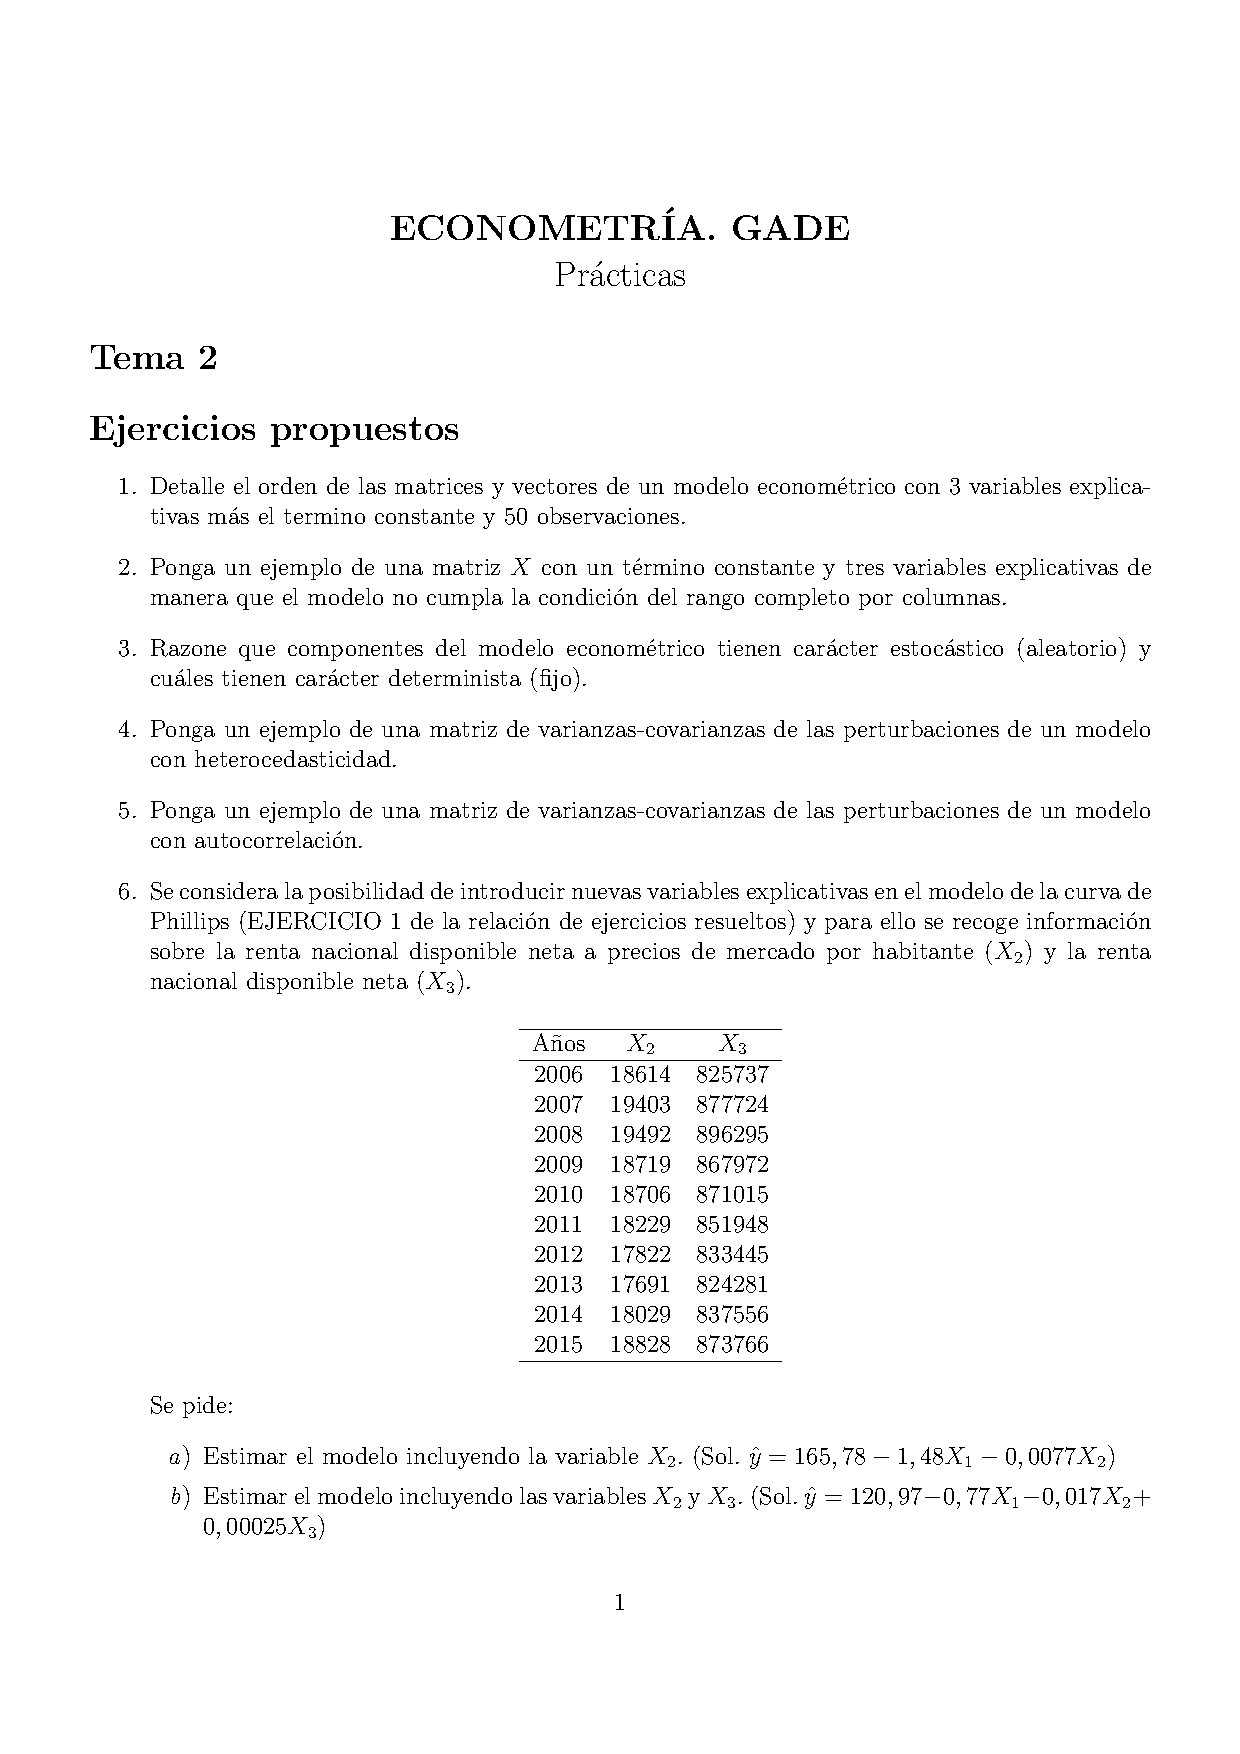
\includepdf[pages=-]{../EjerciciosPropuestos/Tema2_EjerciciosPropuestos.pdf}
\subsection{Tema 3}
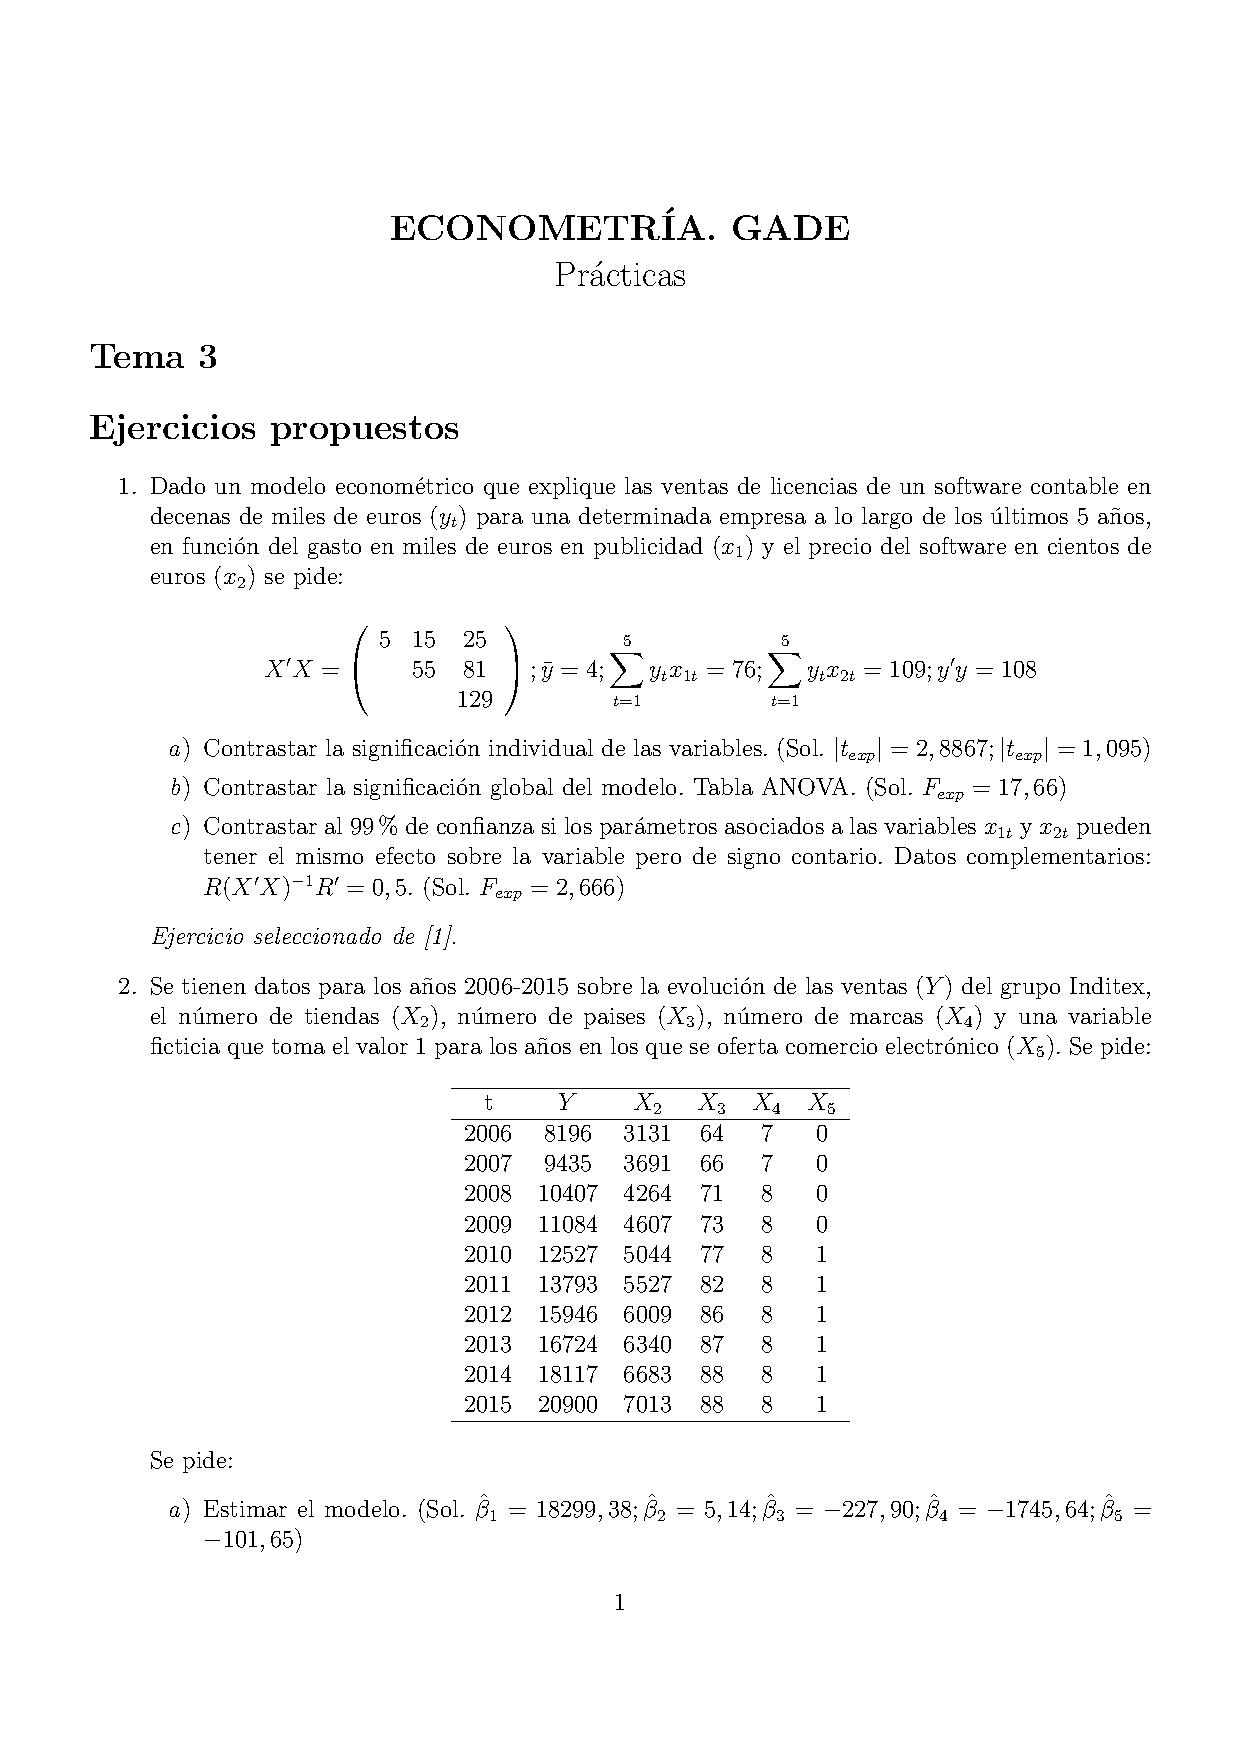
\includepdf[pages=-]{../EjerciciosPropuestos/Tema3_EjerciciosPropuestos.pdf}
\subsection{Tema 4}
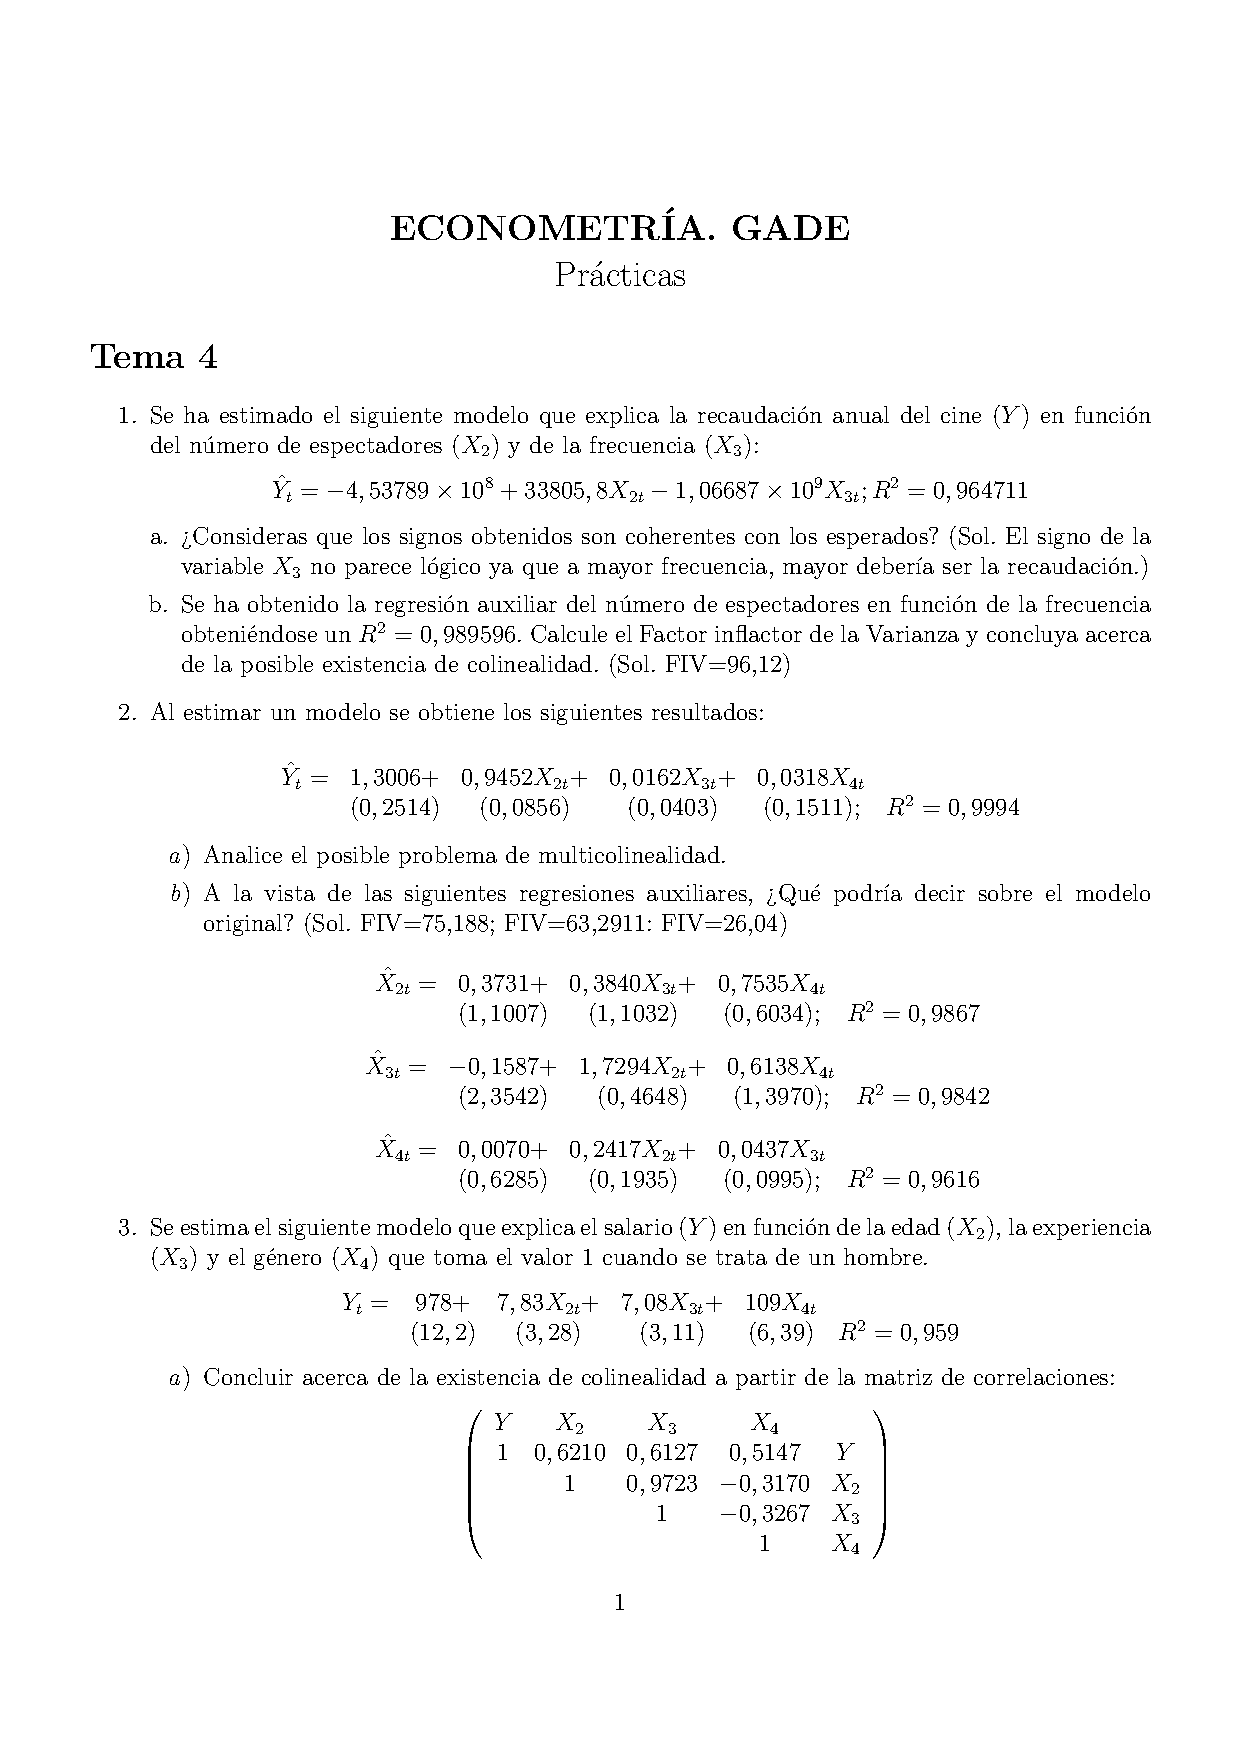
\includepdf[pages=-]{../EjerciciosPropuestos/Tema4_EjerciciosPropuestos.pdf}
\subsection{Tema 5}
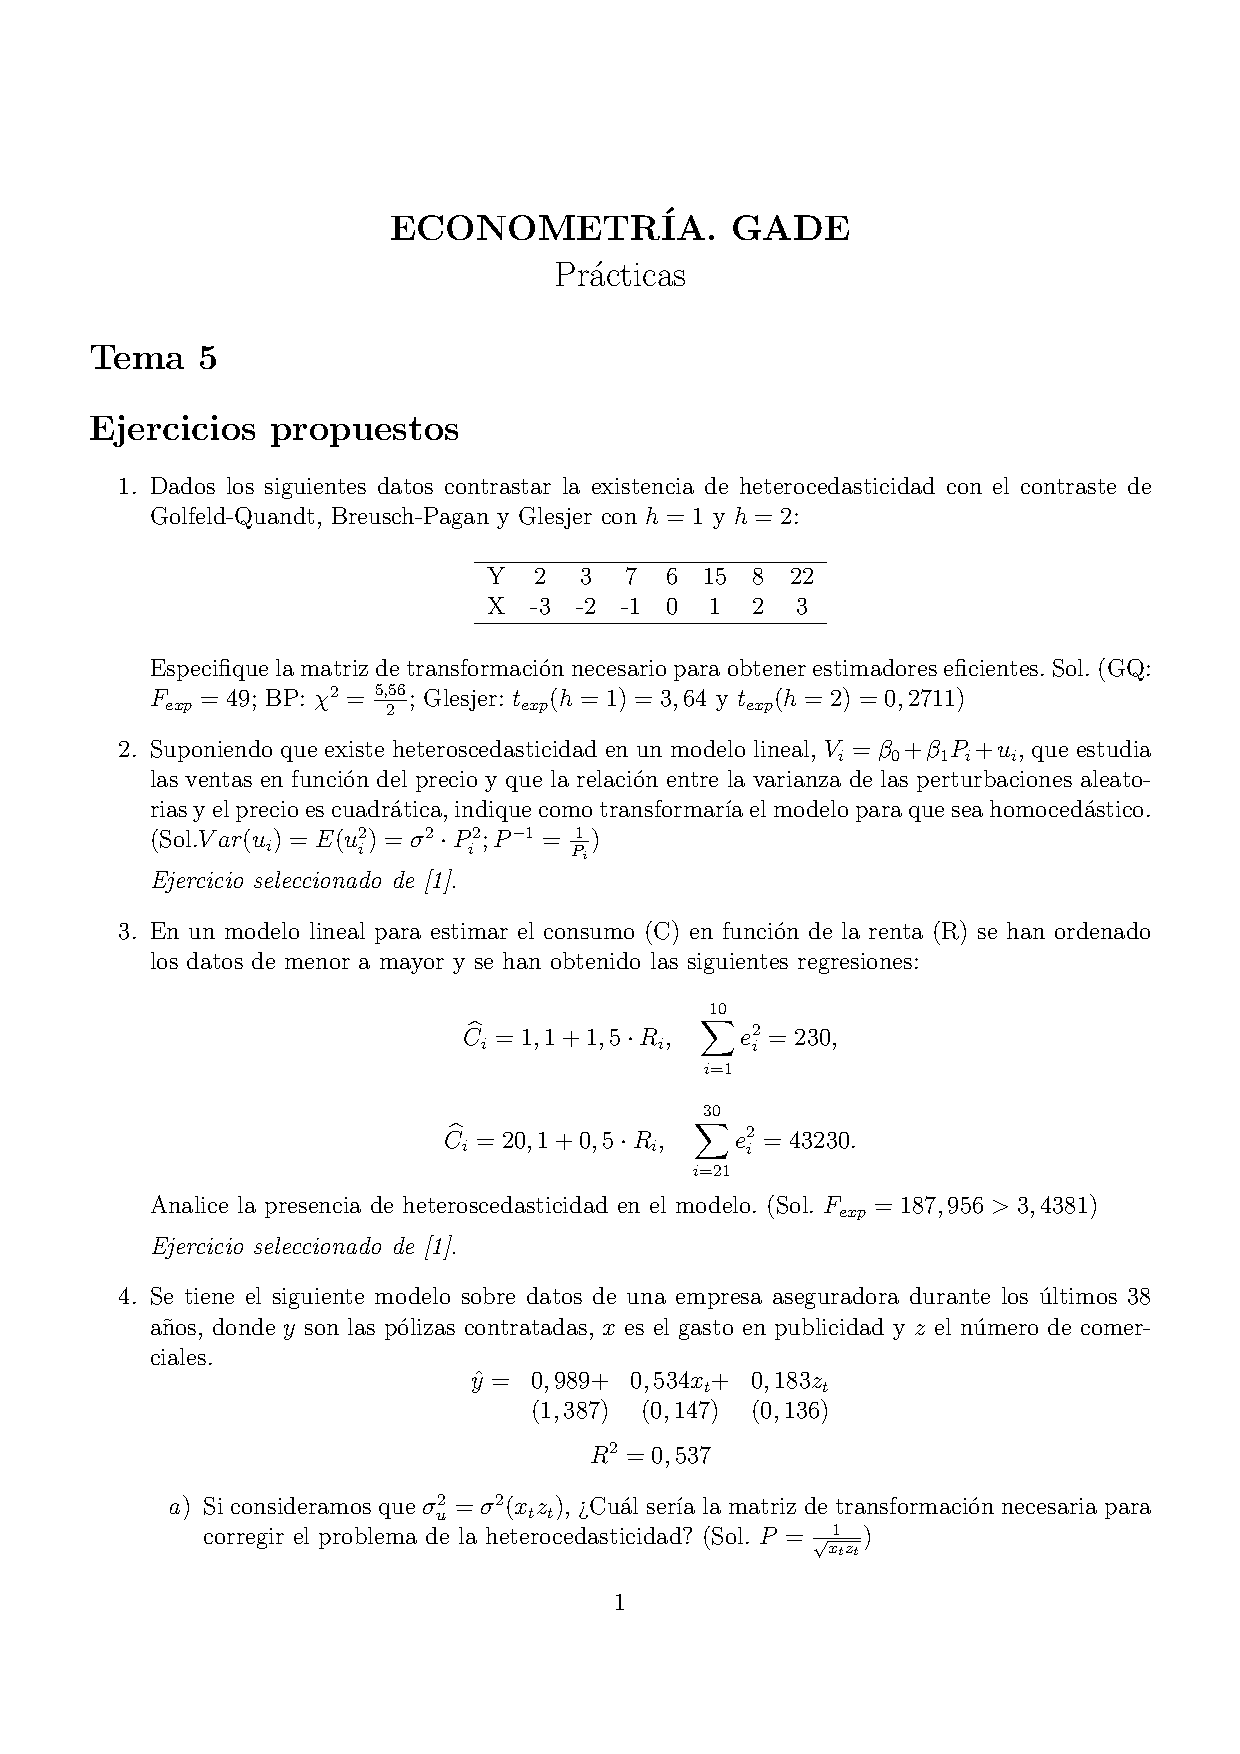
\includepdf[pages=-]{../EjerciciosPropuestos/Tema5_EjerciciosPropuestos.pdf}
\subsection{Tema 6}
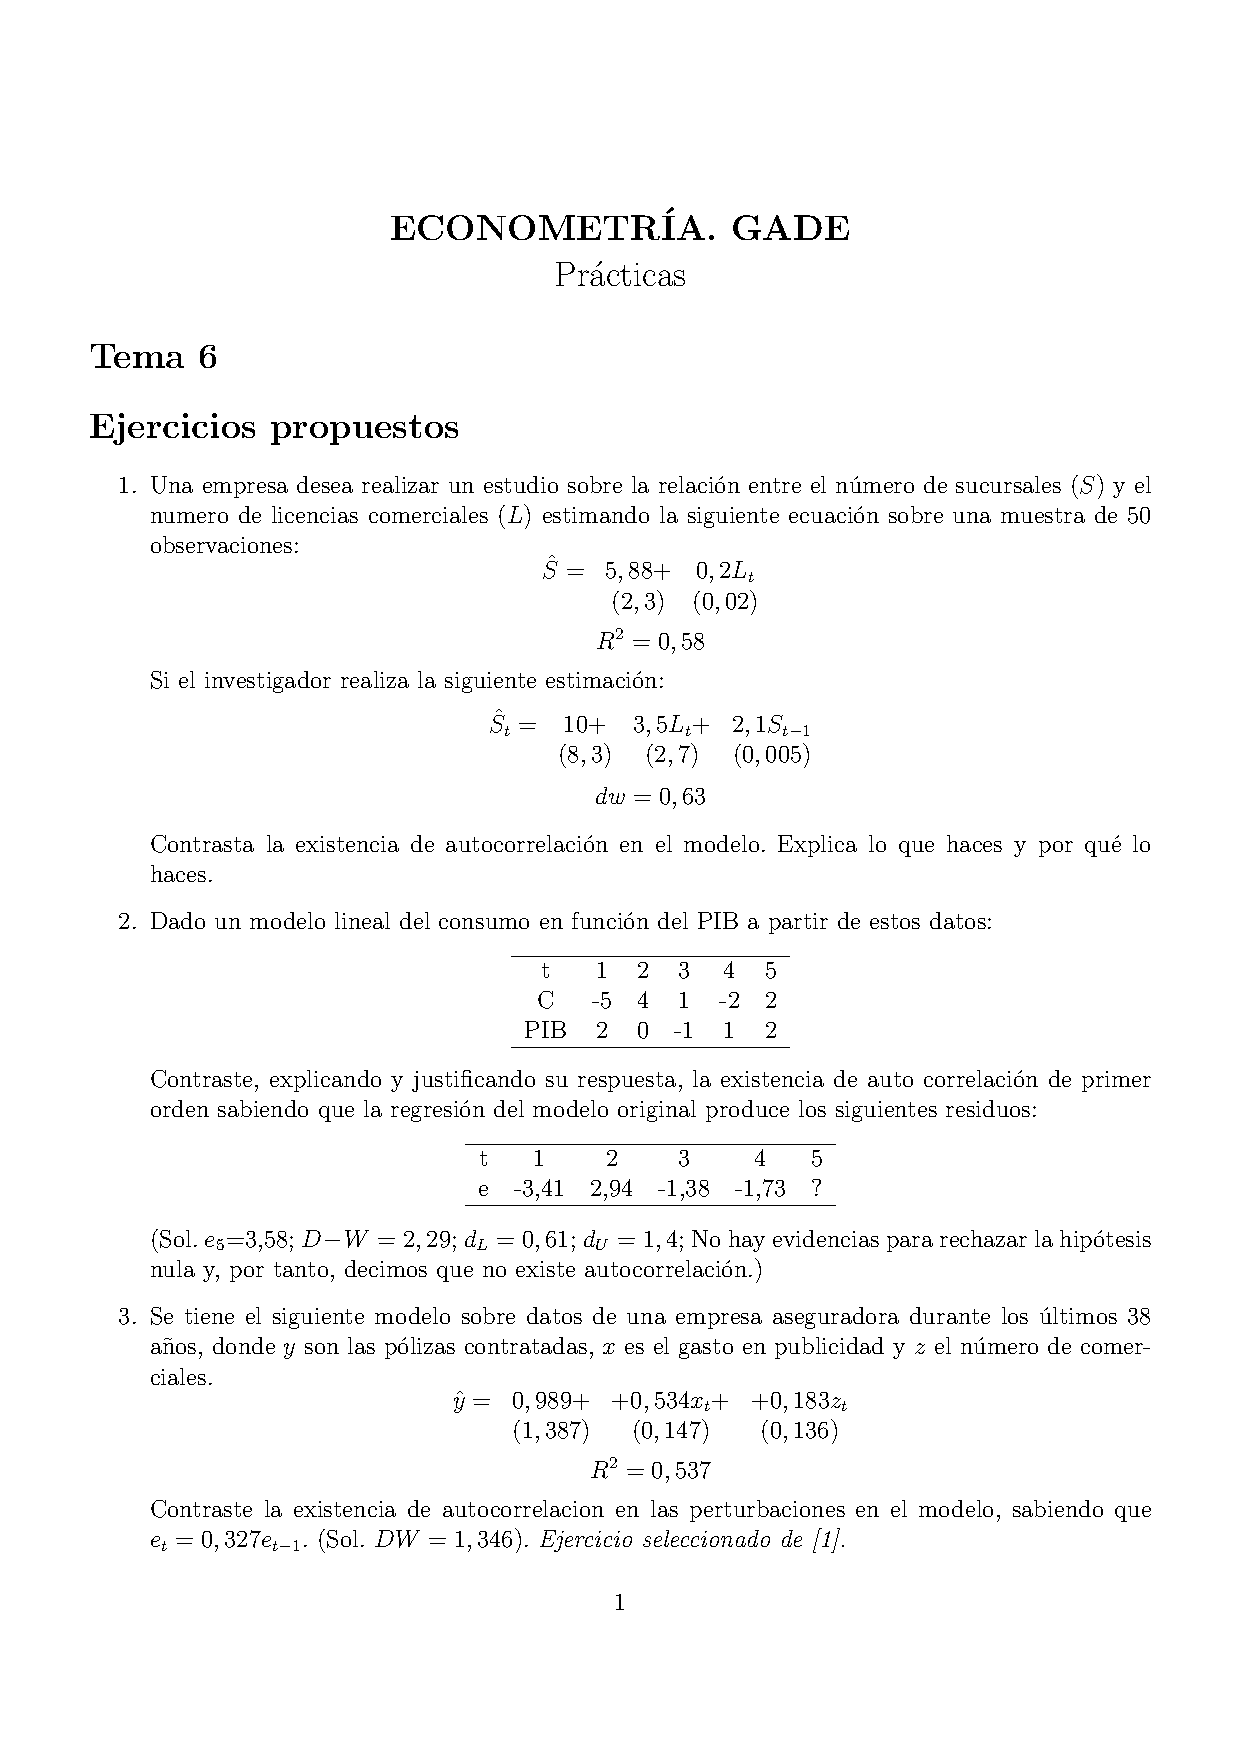
\includepdf[pages=-]{../EjerciciosPropuestos/Tema6_EjerciciosPropuestos.pdf}

\section{Soluciones Ejercicios Propuestos}

\includepdf[pages=-]{../EjerciciosPropuestos/SolucionesEjercicios/FCCEE/build/Ejercicios.pdf}

\section{Ejercicios Resueltos}
\subsection{Tema 2}
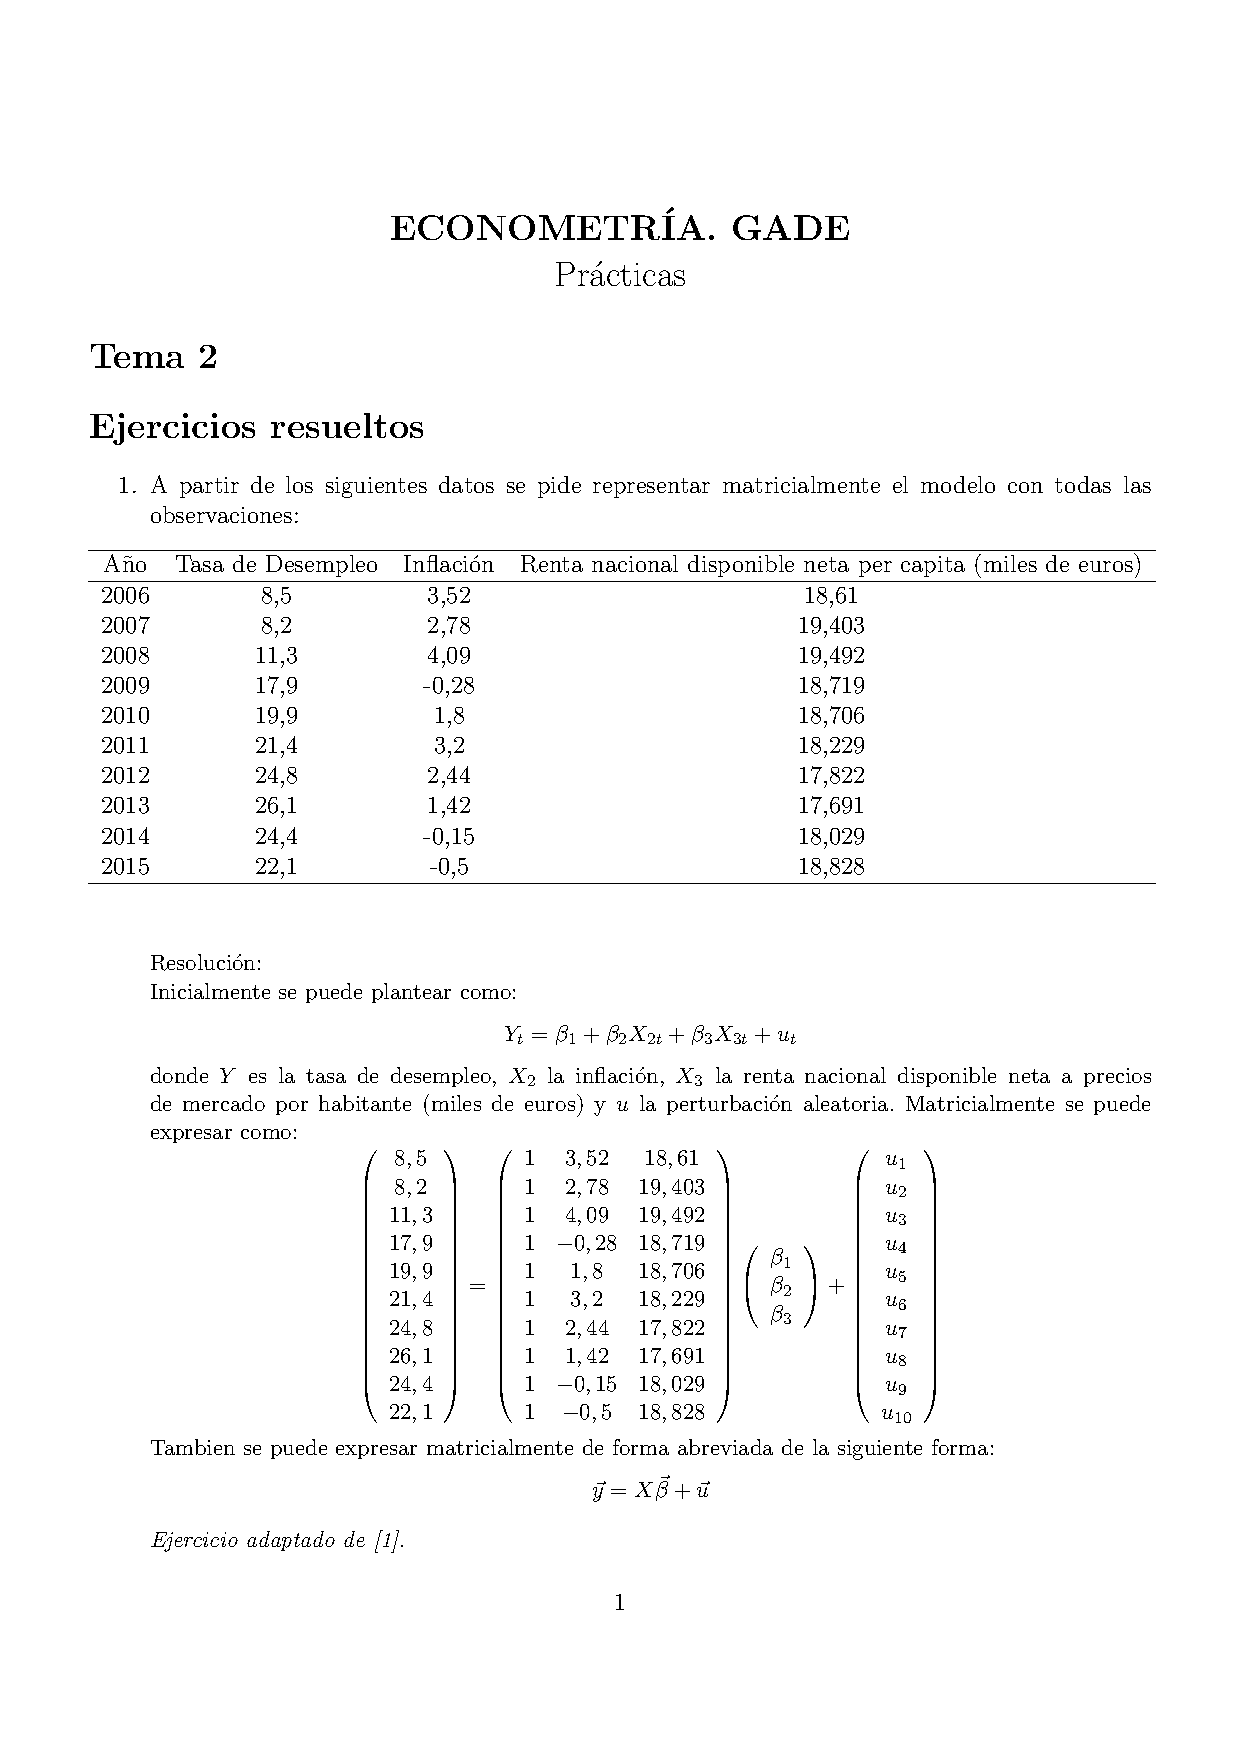
\includepdf[pages=-]{../EjerciciosResueltos/Tema2_EjerciciosResueltos.pdf}
\subsection{Tema 3}
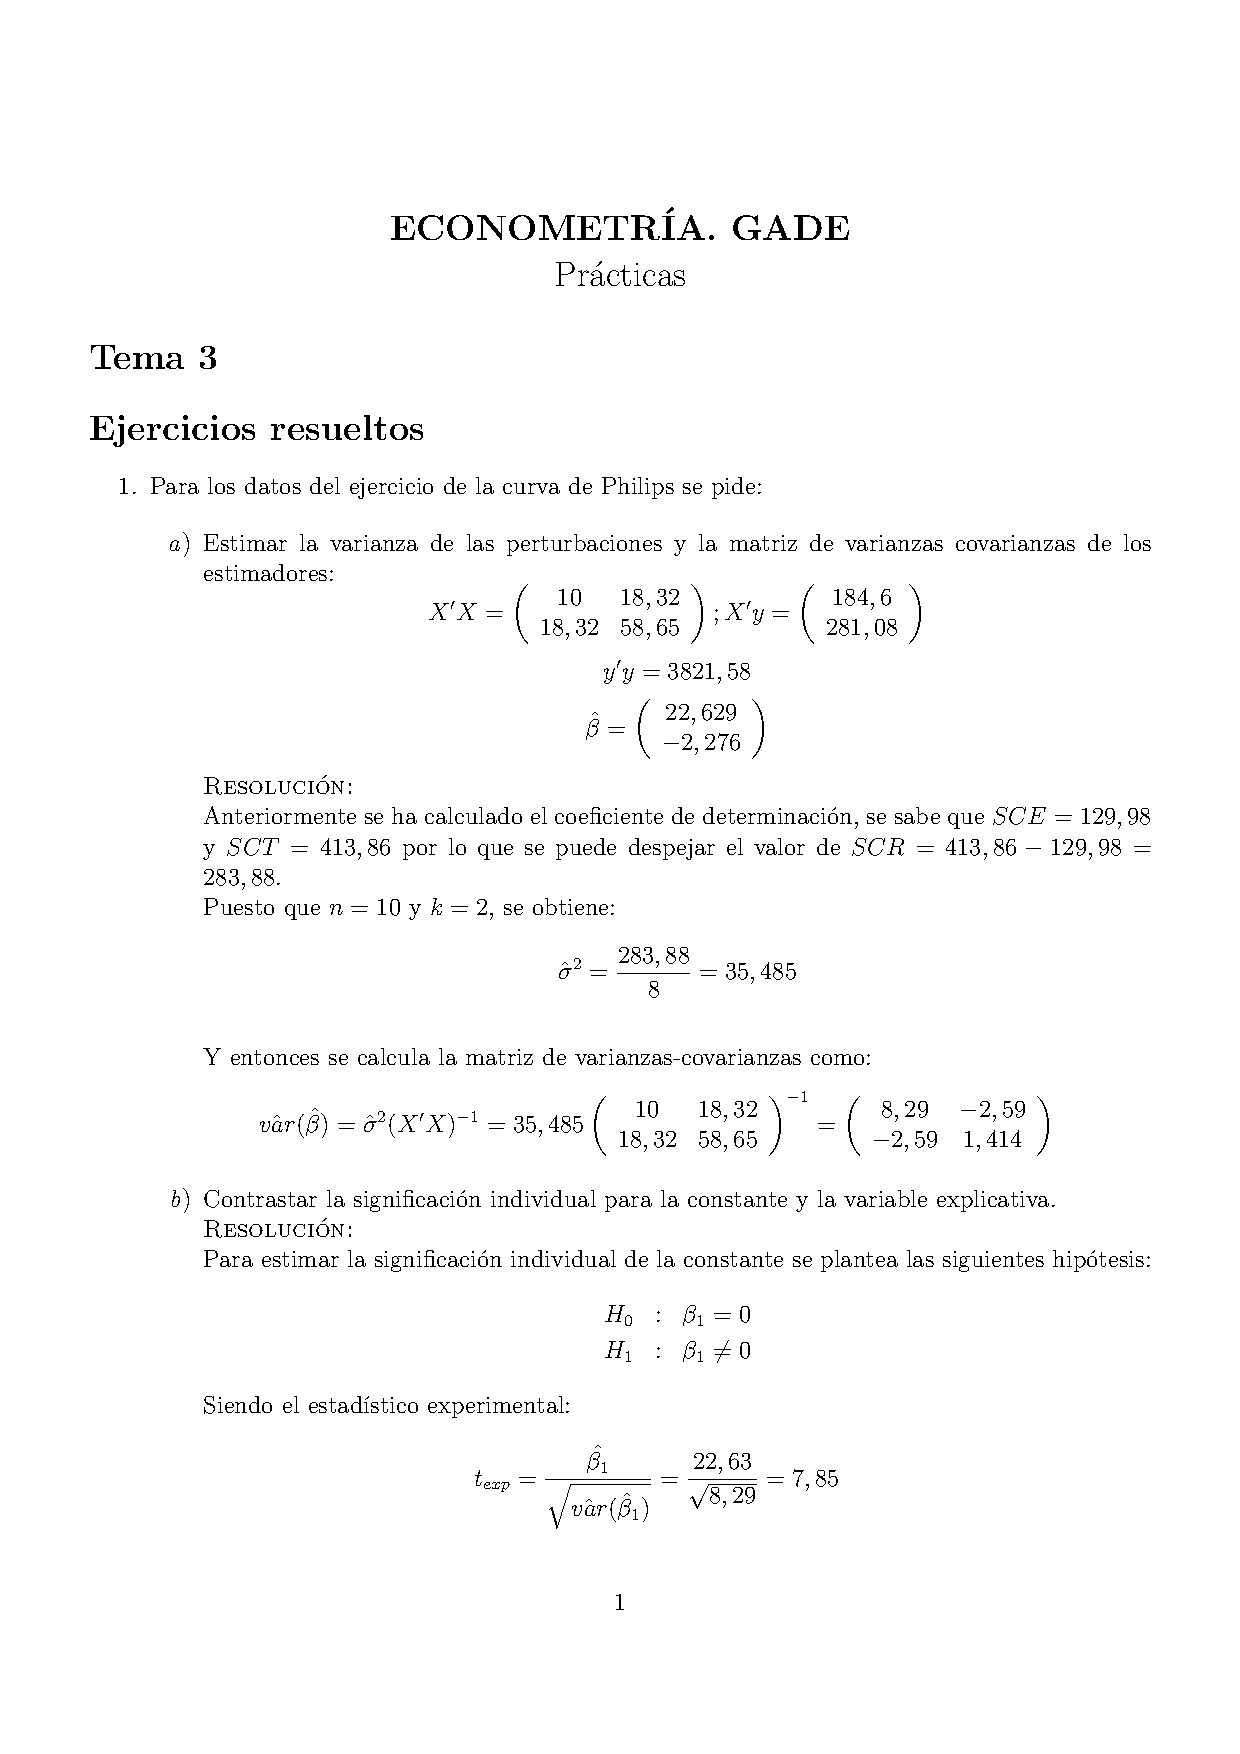
\includepdf[pages=-]{../EjerciciosResueltos/Tema3_EjerciciosResueltos.pdf}
\subsection{Tema 4}
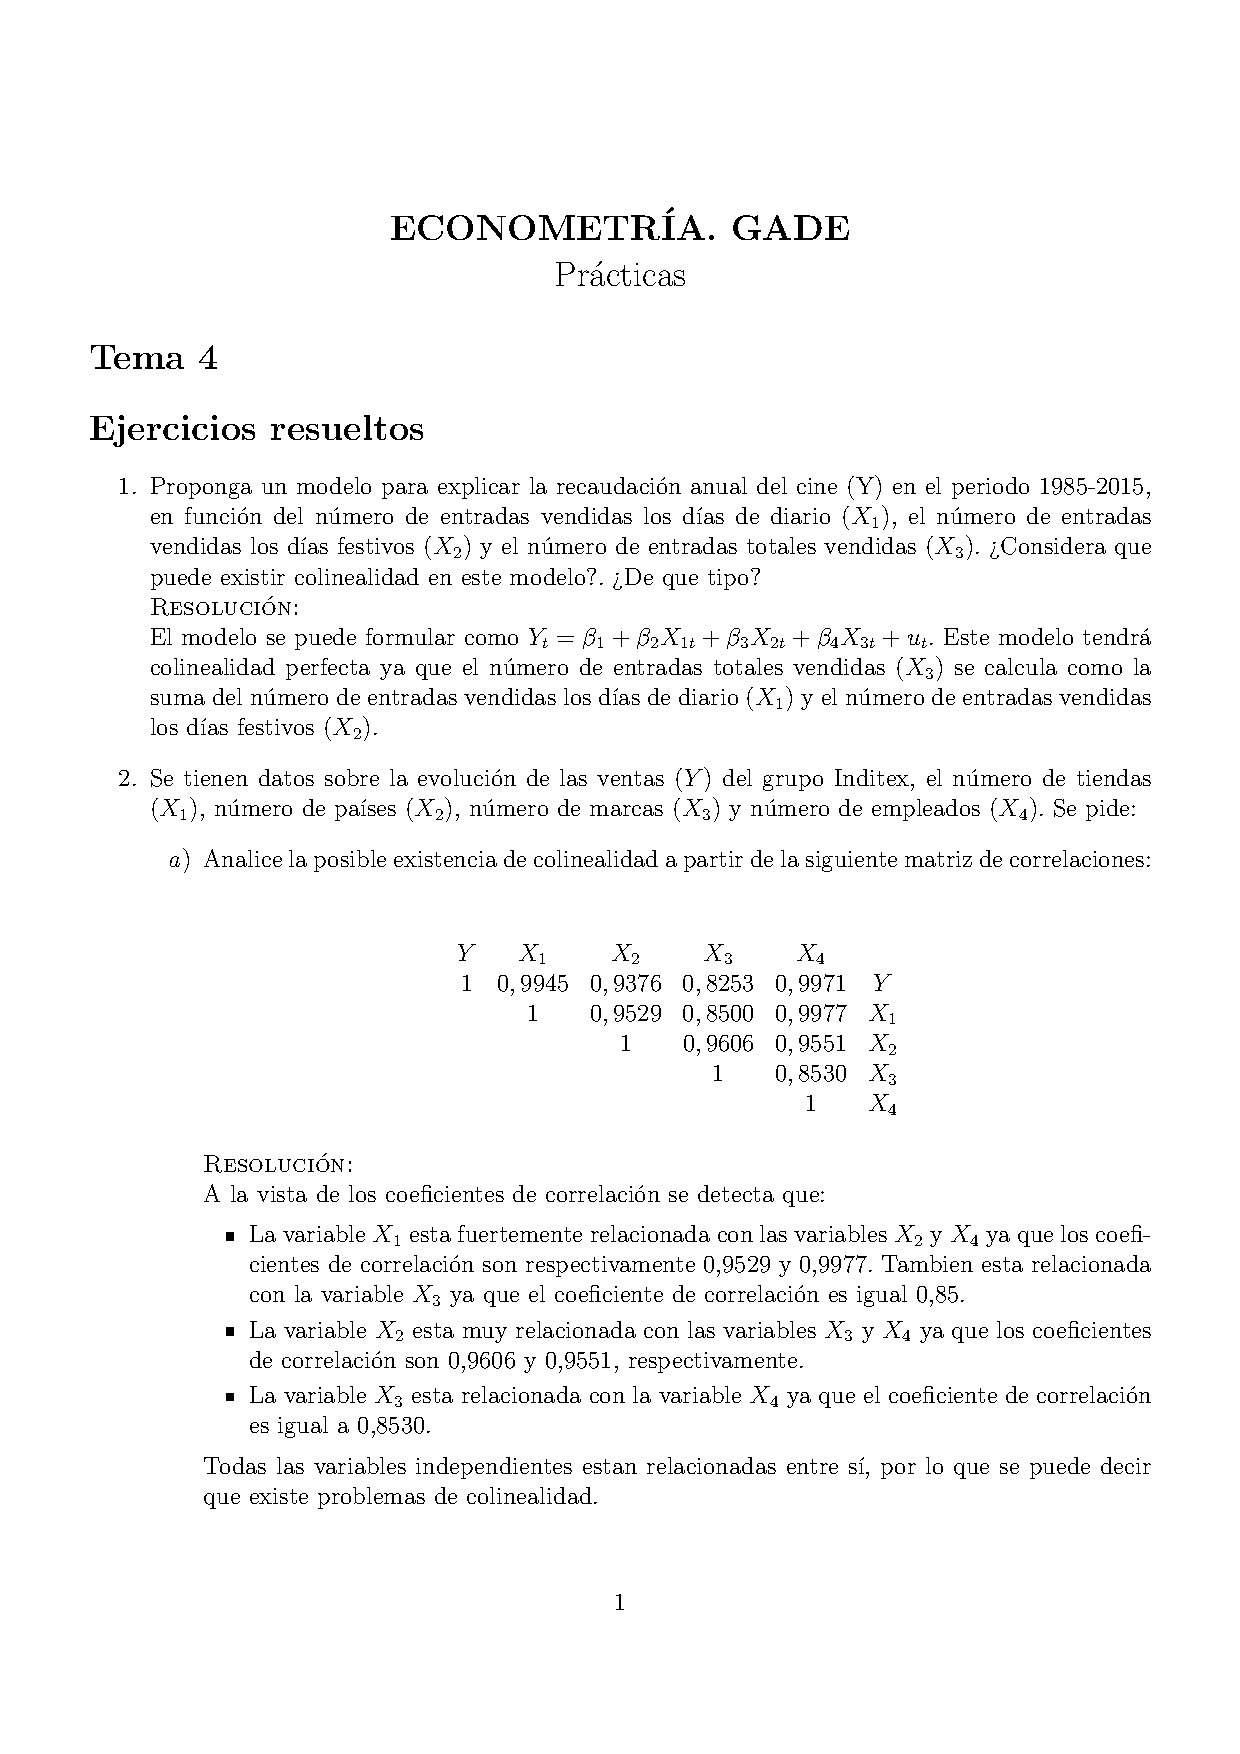
\includepdf[pages=-]{../EjerciciosResueltos/Tema4_EjerciciosResueltos.pdf}
\subsection{Tema 5}
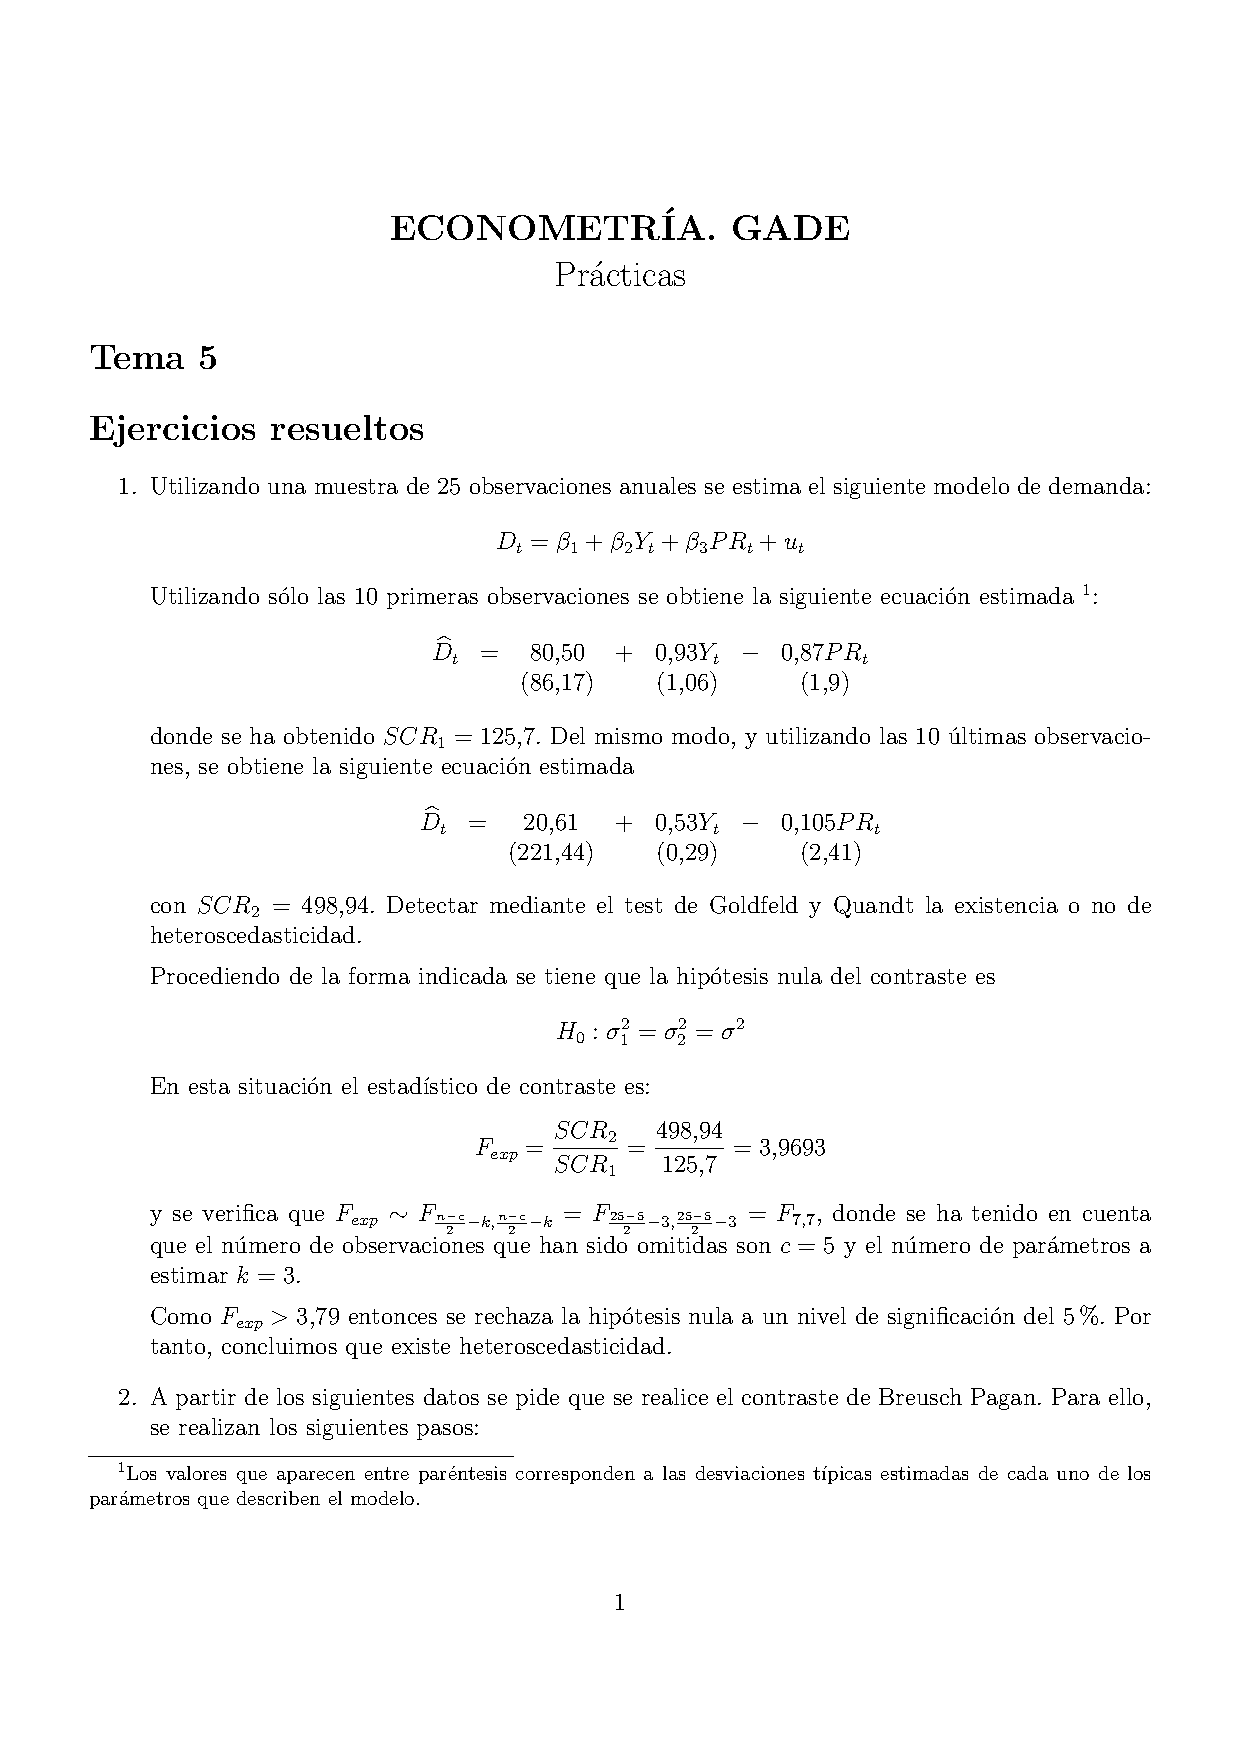
\includepdf[pages=-]{../EjerciciosResueltos/Tema5_EjerciciosResueltos.pdf}
\subsection{Tema 6}
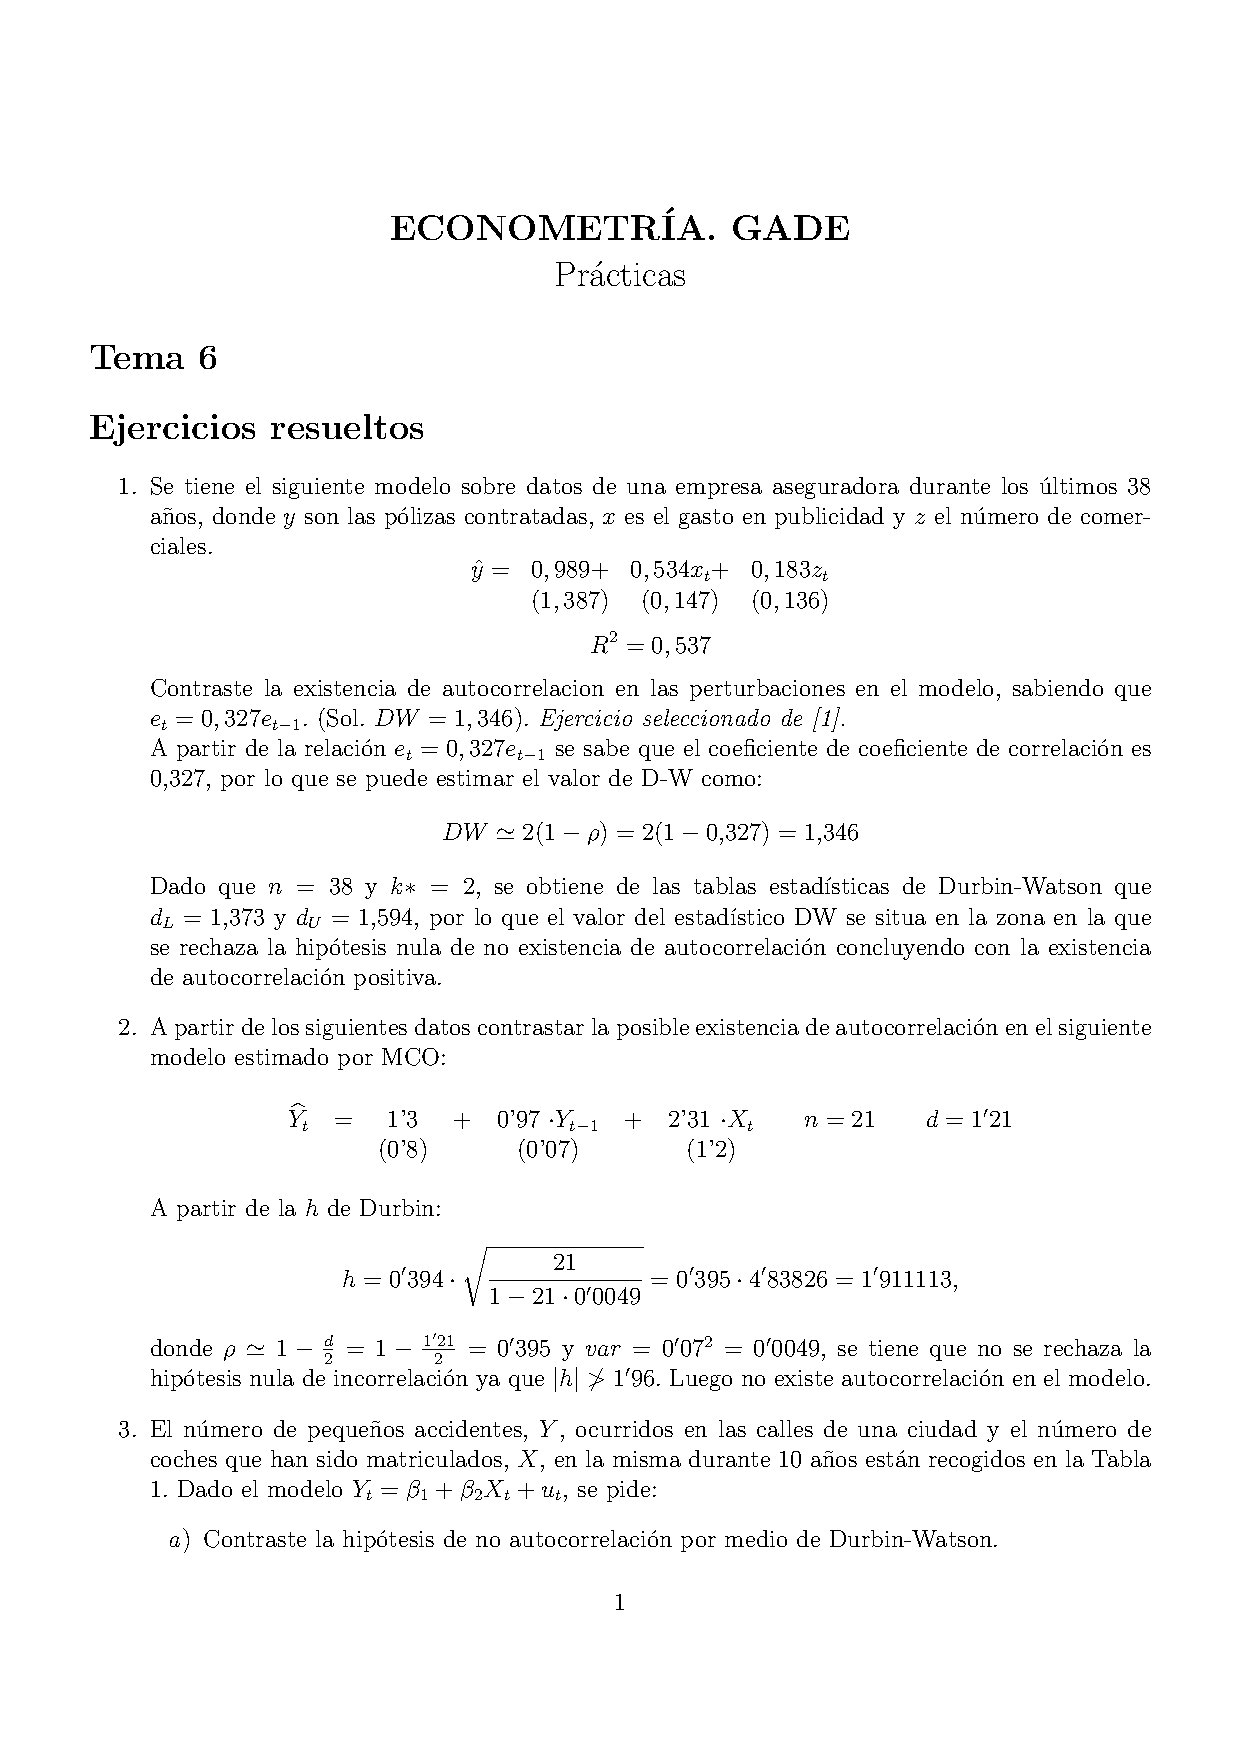
\includepdf[pages=-]{../EjerciciosResueltos/Tema6_EjerciciosResueltos.pdf}
\subsection{Tablas DW}
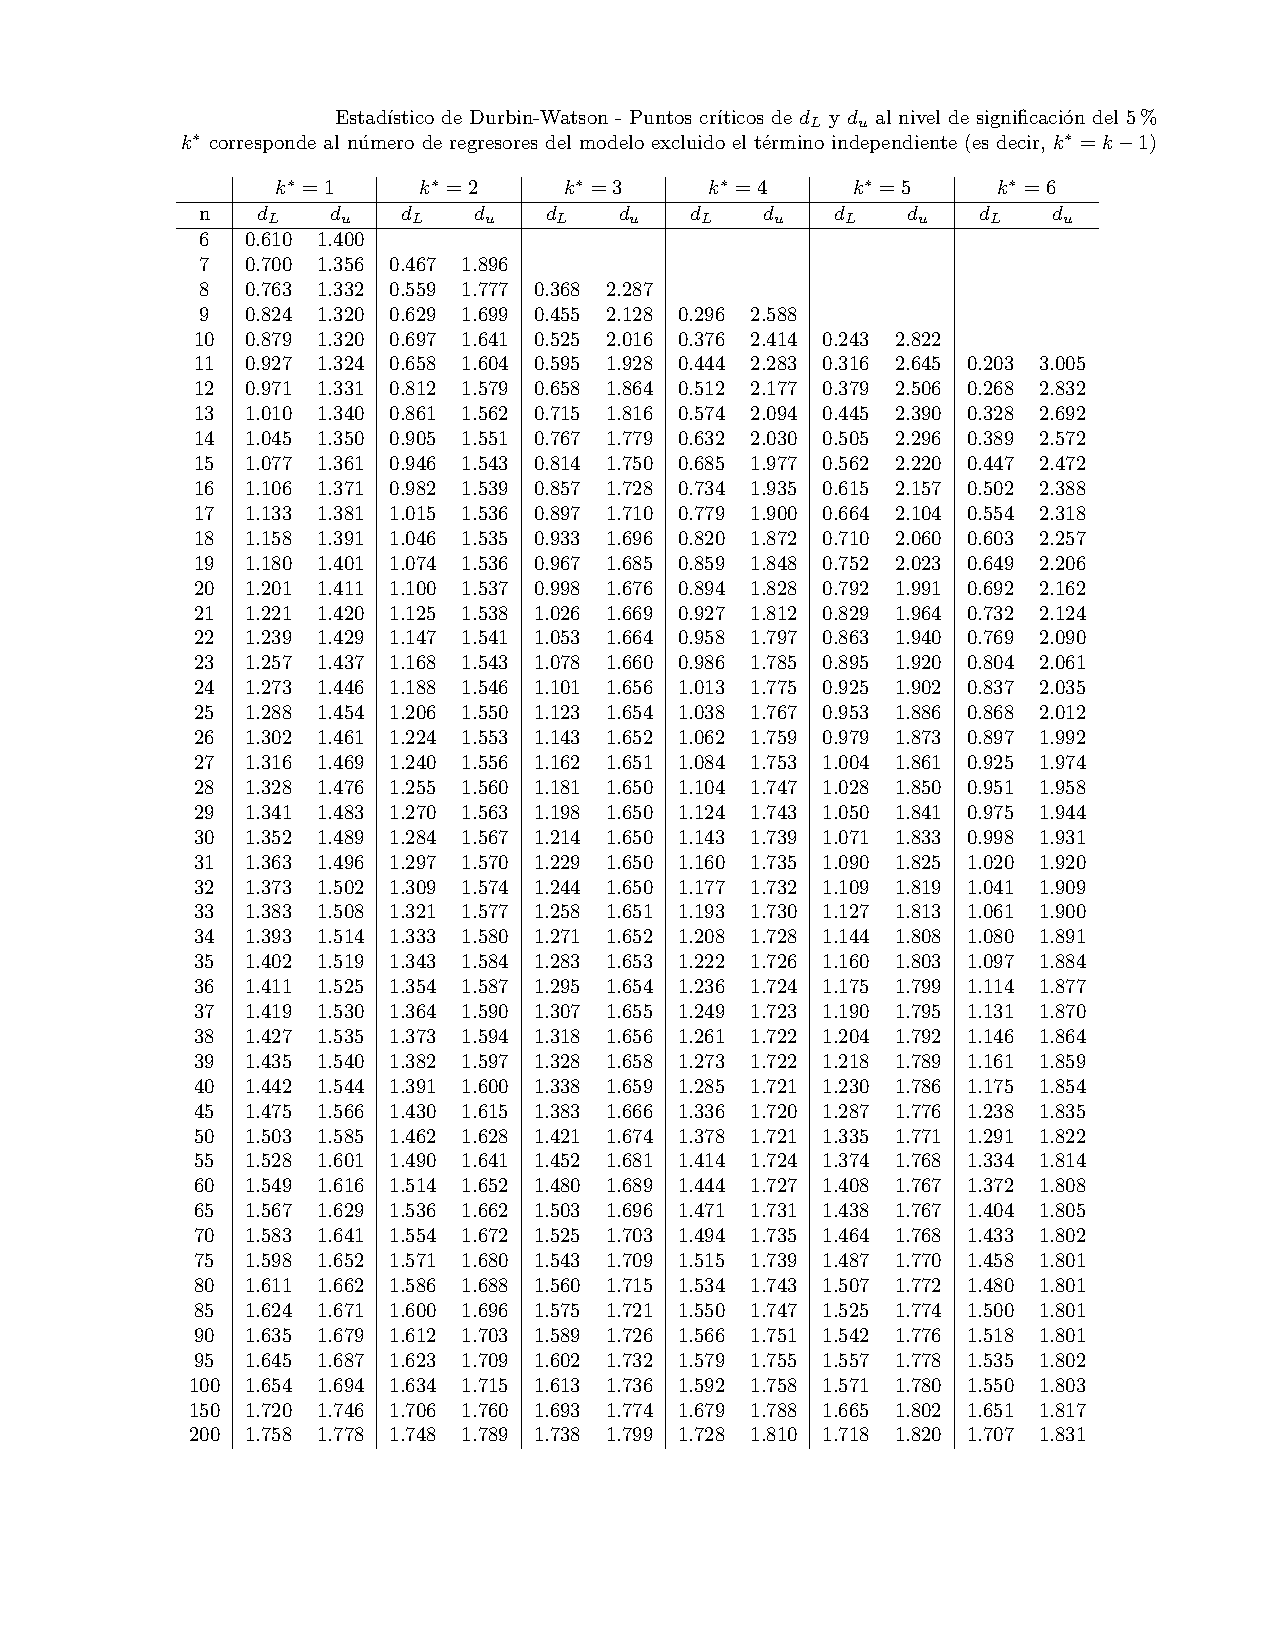
\includepdf[pages=-]{../EjerciciosResueltos/DW.pdf}

\section{Ejemplo Datos Inditex}
%url con los datos en latex en formato xlsx de mi github

\section{Modelo Econométrico}
\subsection{Análisis\_de\_Multicolinealidad}
\includepdf[pages=-]{../Trabajo/Análisis_de_Multicolinealidad.pdf}
\subsection{Modelo\_Preliminar}
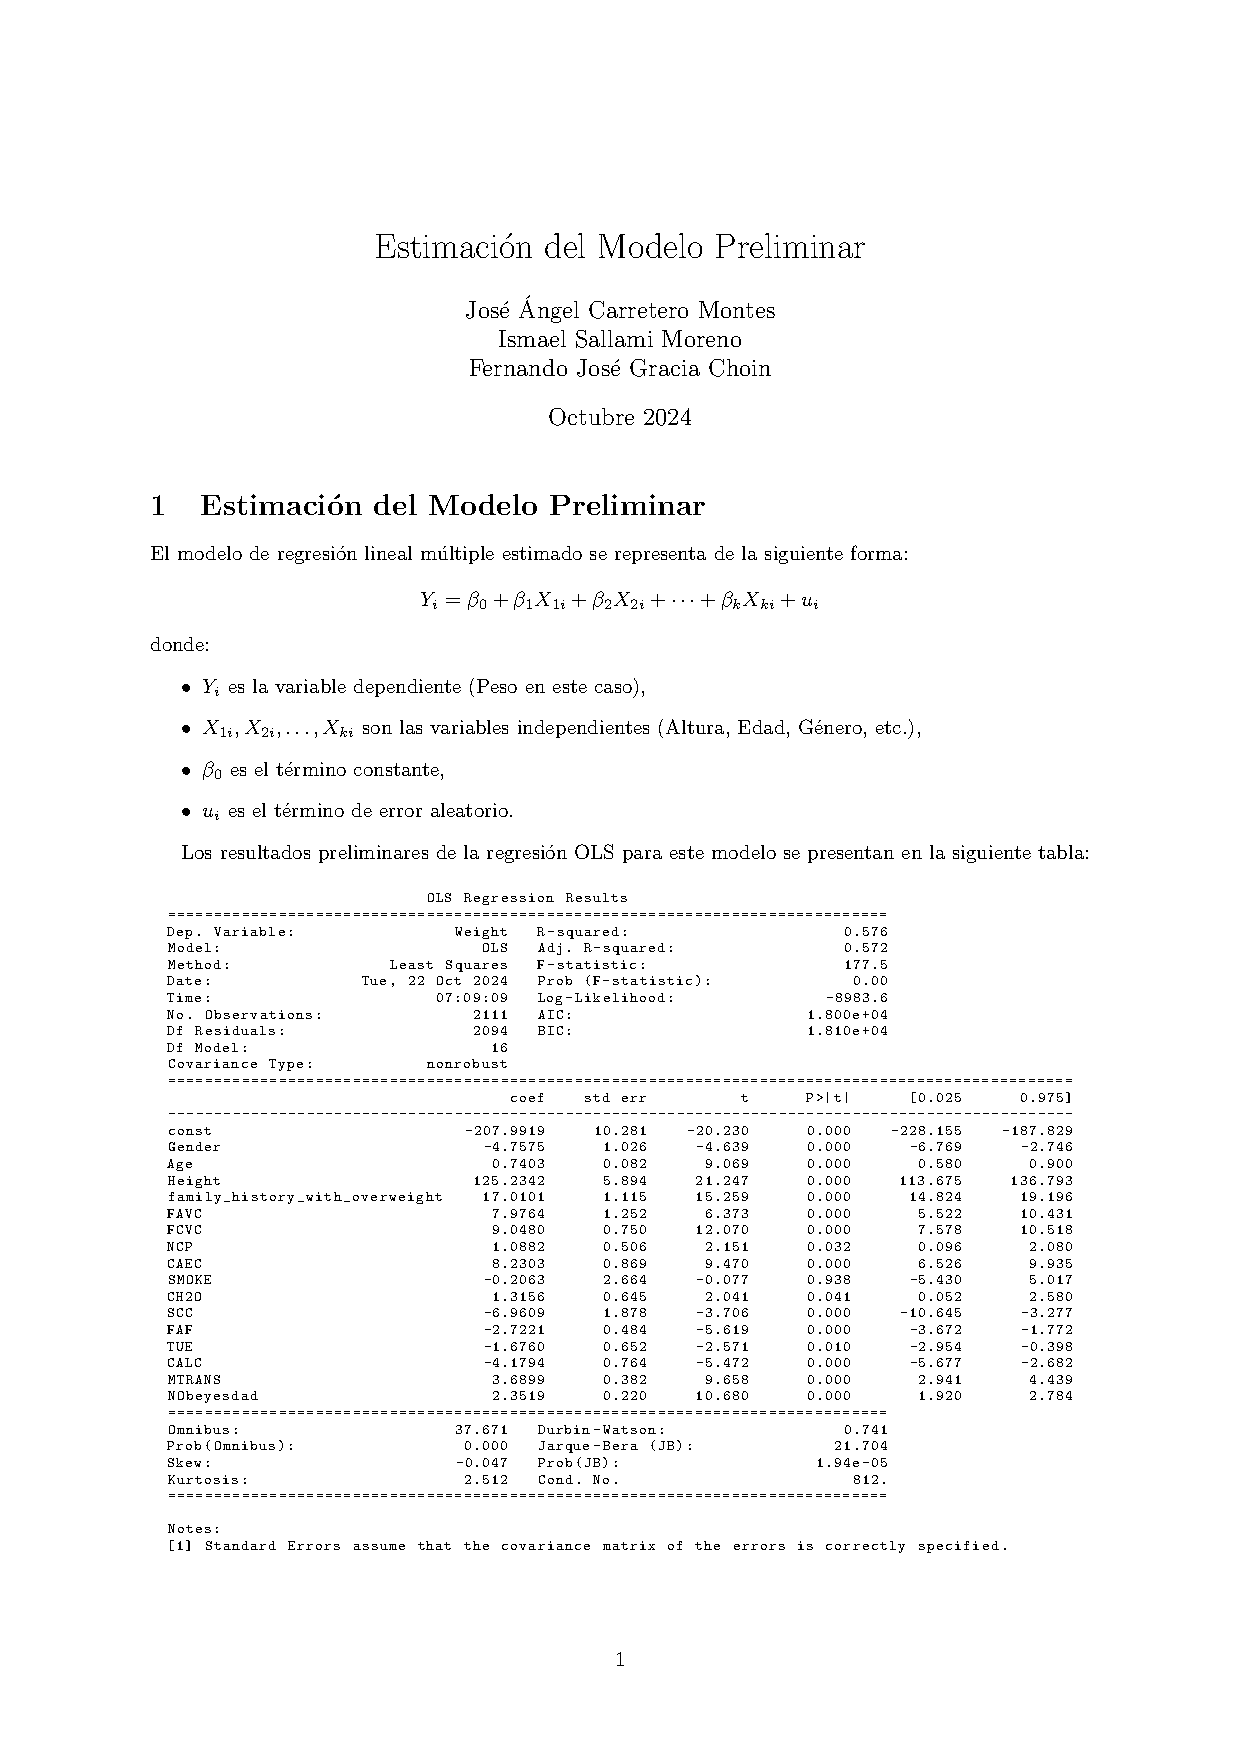
\includepdf[pages=-]{../Trabajo/Modelo_Preliminar.pdf}


\section{Referencias}
\begin{itemize}
    \item Diapositivas de clase.
\end{itemize}


\end{document}
